\section{Quantitative results: discreteness, robustness, and gap statistics}
\label{sec:quantitative}

\subsection{Radial properness and discreteness of \texorpdfstring{$\mathcal{Z}(M)$}{Z(M)}}
The geometric behavior of the point set $\mathcal{Z}(M)\subset\CC$ is largely controlled by the radial character $\rho$.
Recall that by definition (Definition~\ref{def:Z_embedding}) one always has
$$
|\mathcal{Z}(n)|=\rho(n).
$$

\begin{definition}[Radial properness]
\label{def:radial_properness}
We say that a radial character $\rho:M\to\RR_{>0}$ is \emph{proper} if for every $R>0$ the sublevel set
$$
\{n\in M:\ \rho(n)\le R\}
$$
is finite. Equivalently, $\rho(n)\to\infty$ as $n\to\infty$.
\end{definition}

\begin{proposition}[Discreteness of the image]
\label{prop:Z_discrete}
If $\rho$ is proper, then $\mathcal{Z}(M)$ is a discrete subset of $\CC$ (i.e. it intersects every compact set in a finite set), for any phase weights $\beta(p)$.
\end{proposition}

\begin{proof}
Fix a compact $K\subset\CC$. Choose $R>0$ such that $K\subset\{z\in\CC:\ |z|\le R\}$. If $\mathcal{Z}(n)\in K$, then $\rho(n)=|\mathcal{Z}(n)|\le R$, hence $n$ belongs to the finite set $\{m\in M:\rho(m)\le R\}$ by properness.
Therefore $K\cap\mathcal{Z}(M)$ is finite.
\end{proof}

\begin{remark}[Failure under negative prime weights]
If $w(p_0)<0$ for some prime $p_0$, then $\rho_w(p_0^k)=\exp(k w(p_0))\to 0$ as $k\to\infty$.
In particular, $\rho_w$ is not proper and $\mathcal{Z}(M)$ has accumulation at $0$.
The nearest-point projection and kernel normalization statements of Section~\ref{sec:interference} then require modification (or additional conventions).
\end{remark}

\subsection{Projection well-posedness beyond the minimal choice \texorpdfstring{$\rho(n)=n$}{rho(n)=n}}
The nearest-point readout and the soft kernel readout (Definition~\ref{def:nearest_point} and Definition~\ref{def:projection_kernel}) only require quantitative control on how $\rho(n)$ escapes to infinity.

\begin{proposition}[Nearest-point readout under properness]
\label{prop:projection_well_defined_proper}
Assume $\rho$ is proper. Then for every $v\in\CC$ the minimizer set
$$
\operatorname*{Argmin}_{n\in M}\,|v-\mathcal{Z}(n)|
$$
is nonempty and finite. In particular, the nearest-point rule $\pi(v)$ is well-defined (with any fixed tie-breaking convention).
\end{proposition}

\begin{proof}
Fix $v\in\CC$ and set $d_0:=|v-\mathcal{Z}(1)|$.
For all $n\in M$, by the reverse triangle inequality,
$$
|v-\mathcal{Z}(n)|\ge \bigl||\mathcal{Z}(n)|-|v|\bigr|=\bigl|\rho(n)-|v|\bigr|.
$$
If $\rho(n)>|v|+d_0$, then $\bigl|\rho(n)-|v|\bigr|>d_0$, hence $|v-\mathcal{Z}(n)|>d_0$.
Therefore every minimizer lies in the finite set $\{n\in M:\rho(n)\le |v|+d_0\}$, which is finite by properness.
Since the distance function $n\mapsto |v-\mathcal{Z}(n)|$ attains a minimum on a finite set, the minimizer set is nonempty and finite.
\end{proof}

\begin{assumption}[Radial growth for Gaussian normalization]
\label{ass:radial_growth_gaussian}
There exist constants $c>0$ and $s>0$ such that
$$
\rho(n)\ge c\,n^s\qquad (n\in M).
$$
\end{assumption}

\begin{proposition}[Soft projection kernel under polynomial radial growth]
\label{prop:kernel_well_defined_growth}
Assume \ref{ass:radial_growth_gaussian}. Then for every $v\in\CC$ and every $\sigma>0$ the normalizing sum
$$
Z_\sigma(v):=\sum_{n\in M}\exp\!\bigl(-|v-\mathcal{Z}(n)|^2/\sigma^2\bigr)
$$
converges and satisfies $0<Z_\sigma(v)<\infty$.
\end{proposition}

\begin{proof}
Positivity is immediate since each term is positive.
For finiteness, the reverse triangle inequality gives
$$
|v-\mathcal{Z}(n)|\ge \bigl|\rho(n)-|v|\bigr|.
$$
By Assumption~\ref{ass:radial_growth_gaussian}, for all sufficiently large $n$ one has $\rho(n)\ge 2|v|$, hence $\bigl|\rho(n)-|v|\bigr|\ge \rho(n)/2\ge (c/2)n^s$. Therefore for all sufficiently large $n$,
$$
\exp\!\bigl(-|v-\mathcal{Z}(n)|^2/\sigma^2\bigr)\le \exp\!\Bigl(-\frac{c^2}{4\sigma^2}\,n^{2s}\Bigr),
$$
and the series $\sum_{n\ge 1}\exp(-C n^{2s})$ converges for every $C>0$.
Thus $Z_\sigma(v)<\infty$.
\end{proof}

\begin{remark}[Almost-everywhere uniqueness of minimizers]
If $\mathcal{Z}(M)$ is discrete (Proposition~\ref{prop:Z_discrete}), then the set of $v\in\CC$ for which the nearest-point minimizer is not unique is contained in a locally finite union of perpendicular-bisector arcs, and hence has Lebesgue measure zero.
Uniform bounds on the number of minimizers at exceptional $v$ require additional nondegeneracy hypotheses on $\mathcal{Z}(M)$ (e.g. a general-position condition excluding large concyclic subsets).
\end{remark}

\subsection{A robustness bound for window readout and a golden optimality criterion}
Binary window readout stability can be quantified through discrepancy bounds for irrational rotations.
Write the readout as in Section~\ref{sec:readout}:
$$
s_k=\ind_W(x_0+k\alpha),\qquad S_N=\sum_{k=0}^{N-1}s_k.
$$

\begin{theorem}[Ostrowski--Denjoy--Koksma bound for interval counts]
\label{thm:ostrowski_dk}
Let $\alpha=[0;a_1,a_2,\dots]\in(0,1)\setminus\QQ$ and let $q_k$ be the convergent denominators.
Let $W\subset X$ be any interval.
For every $N\in\NN_{>0}$ write the Ostrowski expansion
$$
N=\sum_{k=0}^{m} b_{k} q_k
$$
with digits satisfying \eqref{eq:ostrowski_digits}.
Then for every $x_0\in X$,
$$
\bigl|S_N - N\,\mu(W)\bigr|
\le 2\sum_{k=0}^{m} b_{k}
\le 2\sum_{k=0}^{m} a_{k+1}.
$$
\end{theorem}

\begin{proof}
Let $f:=\ind_W-\mu(W)$. Then $f$ has bounded variation $\mathrm{Var}(f)=2$ and $\int_X f\,d\mu=0$.
For each $k\ge 0$, the Denjoy--Koksma inequality for rotations gives a uniform bound at convergent times:
$$
\left|\sum_{j=0}^{q_k-1} f(x_0+j\alpha)\right|\le \mathrm{Var}(f)=2.
$$
See e.g.~\cite{KatokHasselblatt1995} for the Denjoy--Koksma inequality in the rotation setting.
Now expand $N=\sum_{k=0}^m b_{k} q_k$ and decompose the length-$N$ sum into $b_{m}$ blocks of length $q_m$, then $b_{m-1}$ blocks of length $q_{m-1}$, and so on, using the standard Ostrowski block decomposition.
Applying the $q_k$-time bound to each block yields
$$
\left|\sum_{j=0}^{N-1} f(x_0+j\alpha)\right|
\le 2\sum_{k=0}^m b_{k}.
$$
Since $\sum_{j=0}^{N-1} f(x_0+j\alpha)=S_N-N\mu(W)$, the first inequality follows.
The second inequality follows from the digit bounds in \eqref{eq:ostrowski_digits}, namely $b_0<a_1$ and $b_k\le a_{k+1}$ for $k\ge 1$.
\end{proof}

\begin{corollary}[Golden optimality for a discrepancy proxy]
\label{cor:golden_optimal_discrepancy_proxy}
Fix a depth $m\ge 0$ and consider the quantity
$$
C_m(\alpha):=\sum_{k=0}^{m} a_{k+1},
$$
where $\alpha=[0;a_1,a_2,\dots]$.
Then $C_m(\alpha)\ge m+1$ for every irrational $\alpha$, with equality if and only if $a_i=1$ for all $1\le i\le m+1$.
In particular, among irrational slopes, the golden slope $\alpha=\varphi^{-1}=[0;1,1,1,\dots]$ uniquely minimizes the upper bound in Theorem~\ref{thm:ostrowski_dk} at every finite depth.
\end{corollary}

\begin{proof}
Since each $a_i\in\NN$, one has $a_i\ge 1$ and therefore $C_m(\alpha)\ge m+1$, with equality if and only if $a_i=1$ for $1\le i\le m+1$.
The last statement follows by uniqueness of continued fractions.
\end{proof}

\begin{remark}[Window perturbations]
If $W$ and $W'$ are interval windows, then the Hamming distance between length-$N$ readouts is
$$
\sum_{k=0}^{N-1} |\ind_W(x_0+k\alpha)-\ind_{W'}(x_0+k\alpha)|
=\sum_{k=0}^{N-1}\ind_{W\triangle W'}(x_0+k\alpha),
$$
so Theorem~\ref{thm:ostrowski_dk} gives an explicit stability bound in terms of the window symmetric difference and continued-fraction data.
In the Sturmian/cut-and-project literature, bounded continued fraction coefficients (bounded type) are also the natural Diophantine condition underlying linear repetitivity/linear recurrence for these codings; see e.g.~\cite{LagariasPleasants2003,BugeaudLaurent2005}.
\end{remark}

\subsection{A random-phase model for projection gaps}
In deterministic HPA, the phases $n\mapsto\theta_\times(n)$ are multiplicative (Section~\ref{sec:embedding}) and may exhibit strong arithmetic correlations.
For a solvable baseline, we introduce a random-phase model that isolates geometric constraints from arithmetic structure.

\begin{assumption}[Random-phase spiral model]
\label{ass:random_phase_model}
Assume the minimal radial choice $\rho(n)=n$ and let $(\vartheta_n)_{n\ge 1}$ be i.i.d.\ uniform on $[0,2\pi)$.
Define random points
$$
\mathcal{Z}_{\mathrm{rnd}}(n):=n\,\e^{\iu\vartheta_n}.
$$
\end{assumption}

\begin{definition}[Random-phase distance-to-image and gap]
\label{def:random_gap}
For $v\in\CC$ define
$$
g_{\mathrm{rnd}}(v):=\min_{n\ge 1}|v-\mathcal{Z}_{\mathrm{rnd}}(n)|.
$$
Choose any measurable nearest-point selector $\pi_{\mathrm{rnd}}(v)\in\operatorname*{Argmin}_{n\ge 1}|v-\mathcal{Z}_{\mathrm{rnd}}(n)|$ and set
$$
\delta_{\mathrm{rnd}}(v):=v-\mathcal{Z}_{\mathrm{rnd}}(\pi_{\mathrm{rnd}}(v)).
$$
Then $|\delta_{\mathrm{rnd}}(v)|=g_{\mathrm{rnd}}(v)$.
\end{definition}

\begin{theorem}[A tail bound for random-phase projection gaps]
\label{thm:random_gap_tail}
Assume \ref{ass:random_phase_model}. Fix $v\in\CC$ with $r:=|v|\ge 1$.
Then for every integer $L\in\NN$ with $1\le L\le r$,
$$
\PP\!\left(g_{\mathrm{rnd}}(v)>2L\right)
\le \exp\!\left(-\frac{L^2}{\pi r}\right).
$$
\end{theorem}

\begin{proof}
Let $r=|v|$ and write $v=r\,\e^{\iu\phi}$.
Consider the candidate radii
$$
I_L:=\{n\in\NN:\ |n-r|\le L\}.
$$
For each $n\in I_L$, define the event
$$
E_n:=\left\{|\vartheta_n-\phi|\le \frac{L}{r+L}\ \text{mod }2\pi\right\}.
$$
Since $\vartheta_n$ is uniform, $\PP(E_n)=\frac{2(L/(r+L))}{2\pi}=\frac{L}{\pi(r+L)}$.
Moreover, on $E_n$ one has
$$
|v-\mathcal{Z}_{\mathrm{rnd}}(n)|
\le |r-n| + n\,|\,\e^{\iu\phi}-\e^{\iu\vartheta_n}\,|
\le L + n\cdot|\phi-\vartheta_n|
\le L + (r+L)\frac{L}{r+L}
= 2L,
$$
for $n\in I_L$, hence $g_{\mathrm{rnd}}(v)\le 2L$ whenever at least one $E_n$ occurs.

The events $(E_n)_{n\in I_L}$ are independent, so
$$
\PP\!\left(\bigcap_{n\in I_L} E_n^c\right)
=\prod_{n\in I_L}\left(1-\frac{L}{\pi(r+L)}\right)
\le \exp\!\left(-\frac{L}{\pi(r+L)}\,|I_L|\right).
$$
Since $1\le L\le r$, one has $|I_L|\ge 2L$ and $(r+L)\le 2r$, so
$$
\PP\!\left(\bigcap_{n\in I_L} E_n^c\right)\le \exp\!\left(-\frac{L}{\pi(r+L)}\,2L\right)\le \exp\!\left(-\frac{L^2}{\pi r}\right),
$$
which implies the claimed tail bound.
\end{proof}

\begin{remark}[Interpretation]
Theorem~\ref{thm:random_gap_tail} shows that in a random-phase model the typical gap scale grows like $r^{1/2}$, so the \emph{relative} mismatch $g_{\mathrm{rnd}}(v)/|v|$ decays like $r^{-1/2}$.
This provides a quantitative baseline for the slogan that additive readout becomes more accurate at large radii, while remaining intrinsically lossy at finite resolution.
\end{remark}

\subsection{Numerical experiments (reproducible)}
Section~\ref{sec:interference} defines the deterministic gap $\delta(a,b)$ and the distance function $g(v)$.
Figures in this subsection are generated by the repository script
$$
\texttt{docs/papers/2025\_holographic\_polar\_arithmetic/scripts/generate\_figures.py}
$$
which writes outputs into
$$
\texttt{docs/papers/2025\_holographic\_polar\_arithmetic/images/}.
$$
Unless stated otherwise, the experiments use $\rho(n)=n$.
We sample $(a,b)$ uniformly from $\{1,\dots,5000\}^2$ and compute the nearest-point readout against $\{1,\dots,20000\}$.

\paragraph{Phase choices.}
The script instantiates the following explicit models:
\begin{itemize}
    \item \textbf{Log-phase:} $\theta_\times(n)\equiv \beta_0\log n\ (\mathrm{mod}\ 2\pi)$ with $\beta_0=4$.
    \item \textbf{$\Omega$-phase:} $\theta_\times(n)\equiv \beta_1\,\Omega(n)\ (\mathrm{mod}\ 2\pi)$ with $\beta_1=2$ and $\Omega(n)$ the total number of prime factors counted with multiplicity.
    \item \textbf{Random prime phase:} independent $\beta(p)\sim\mathrm{Unif}[0,2\pi)$ for primes $p\le 20000$ (fixed seed), extended multiplicatively via $\theta_\times(n)=\sum_p a_p(n)\beta(p)$.
\end{itemize}

\begin{figure}[t]
    \centering
    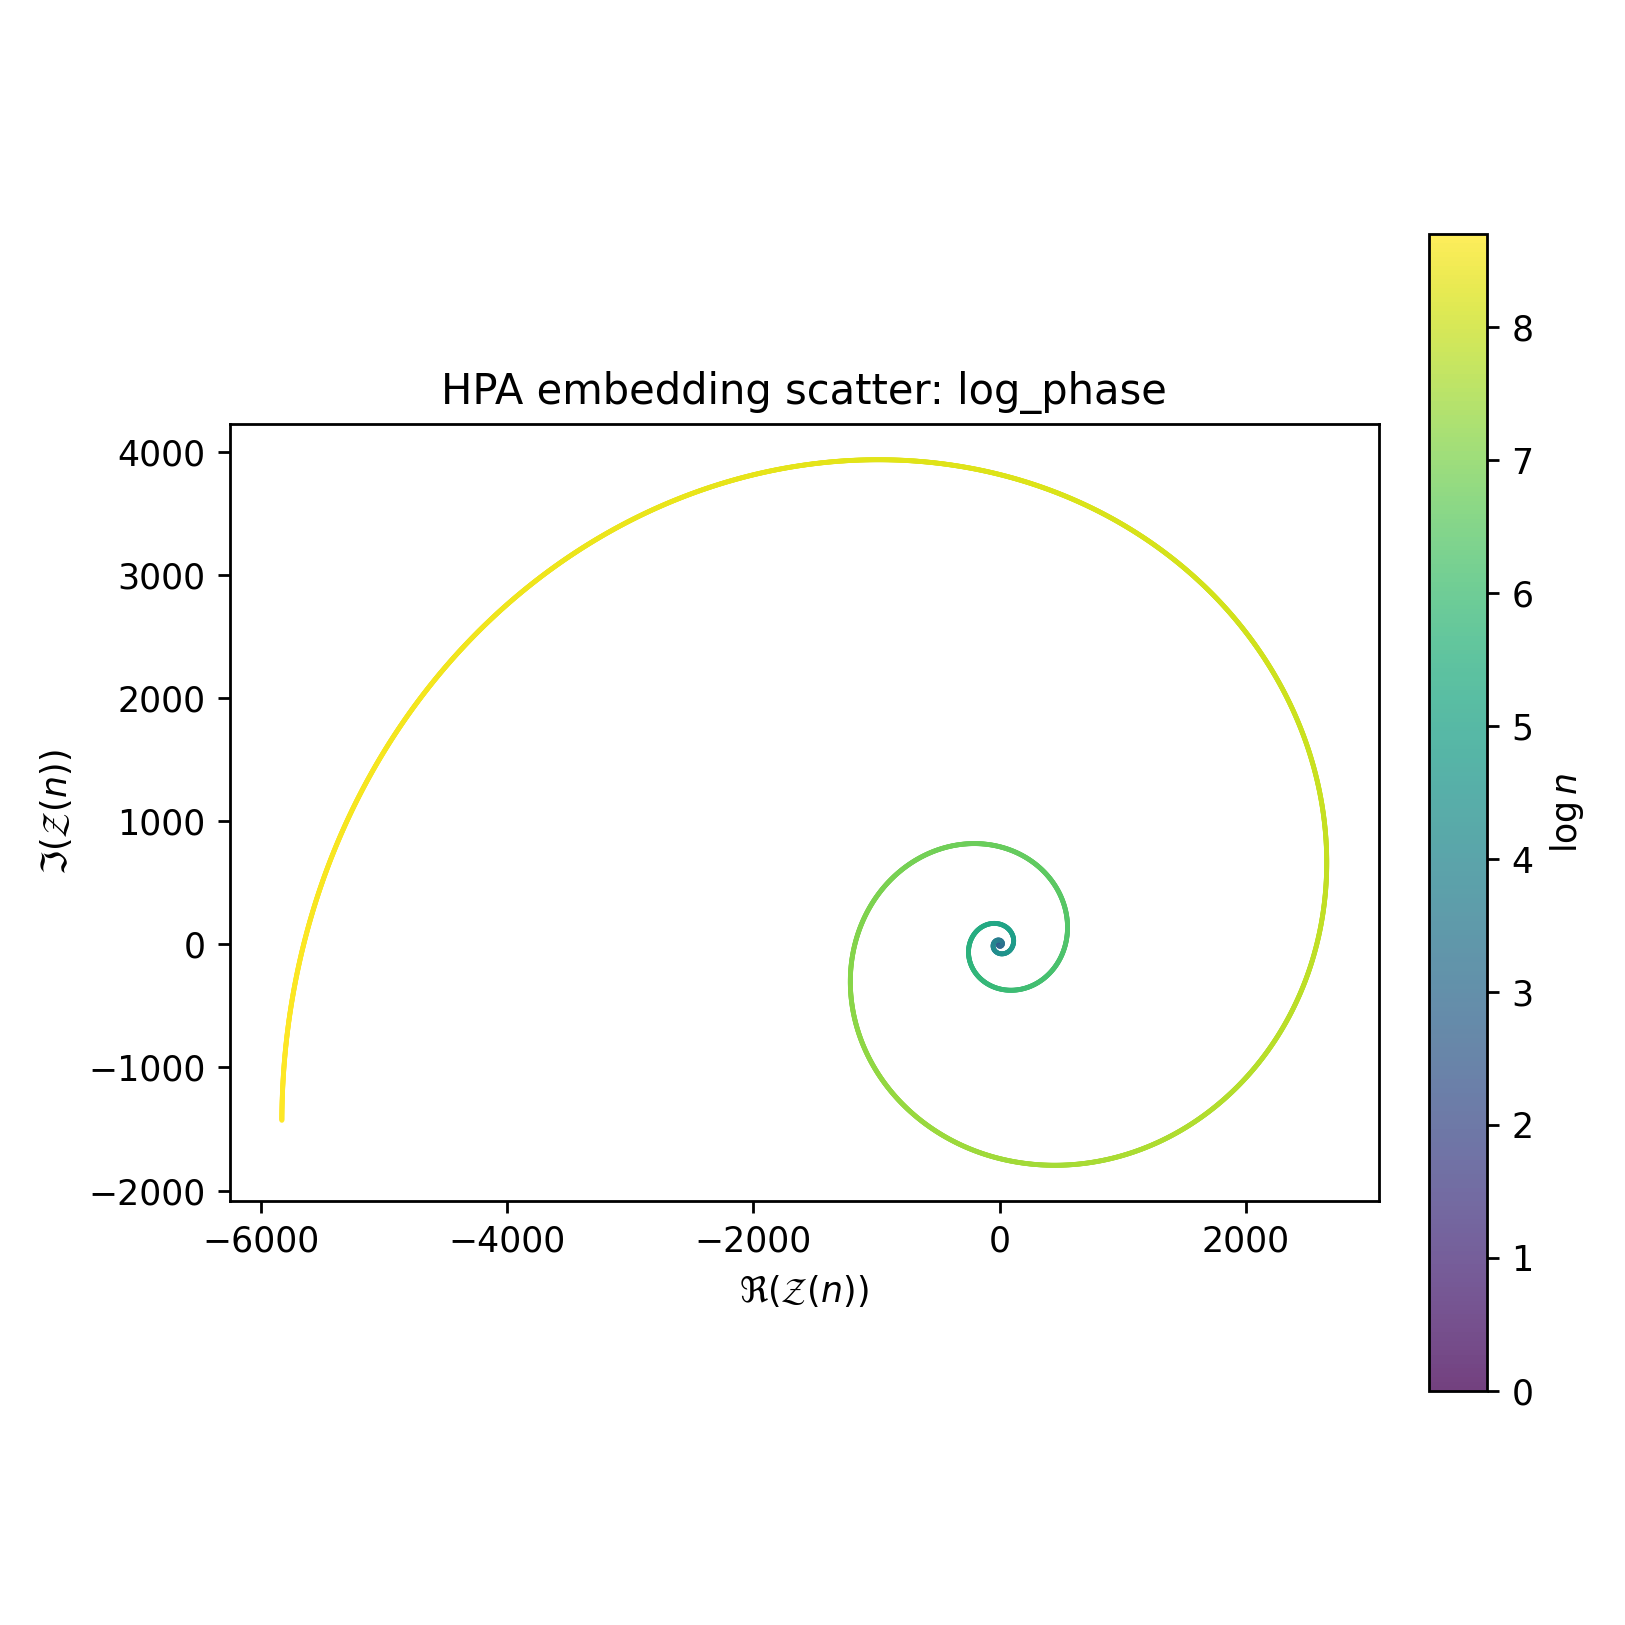
\includegraphics[width=0.32\textwidth]{images/hpa_Z_scatter_log_phase.png}\hfill
    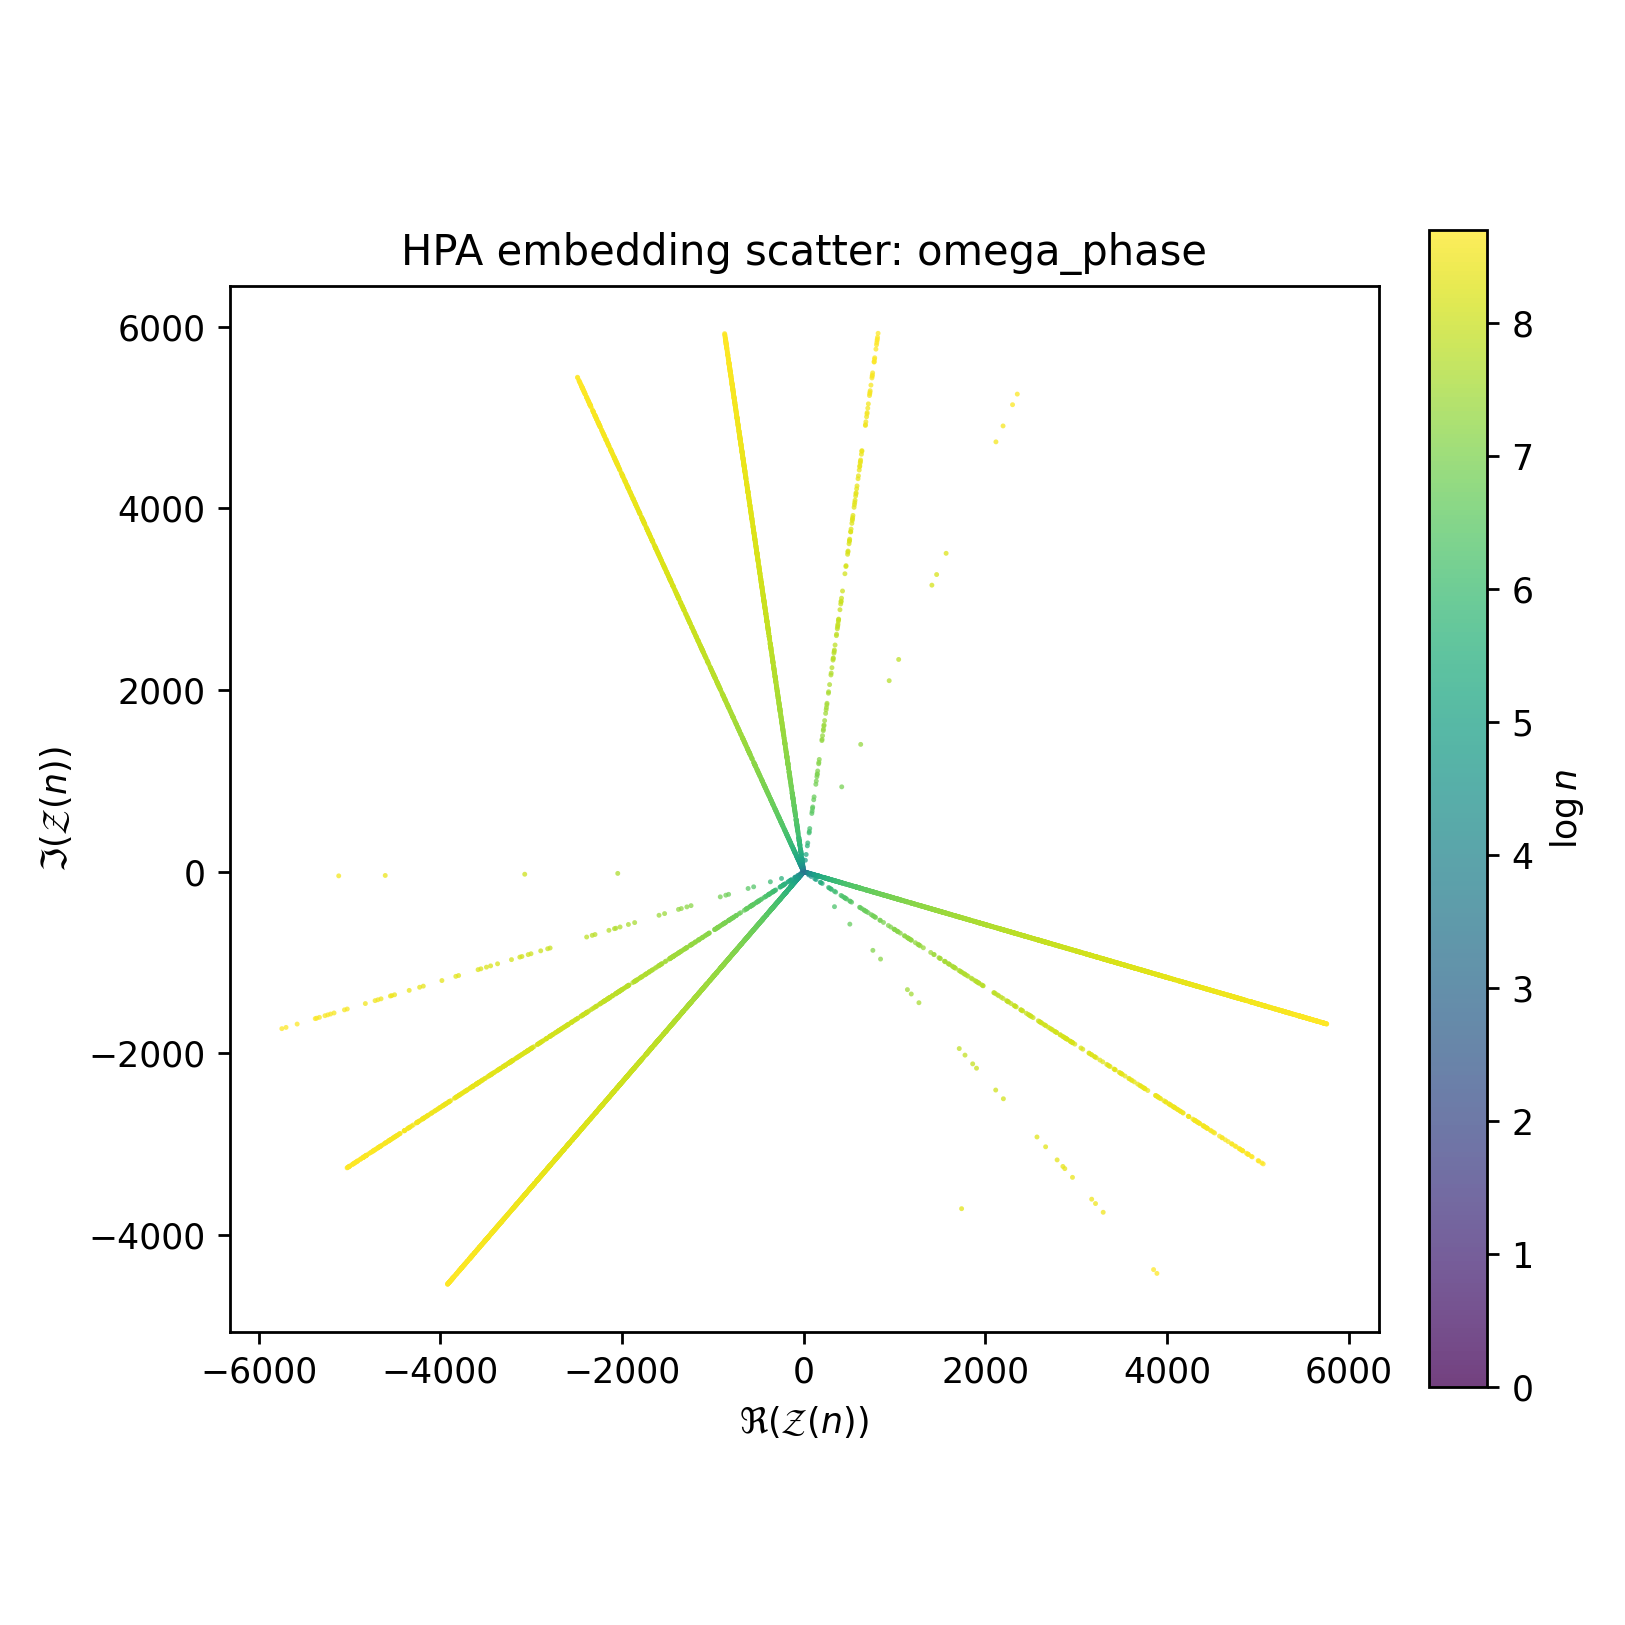
\includegraphics[width=0.32\textwidth]{images/hpa_Z_scatter_omega_phase.png}\hfill
    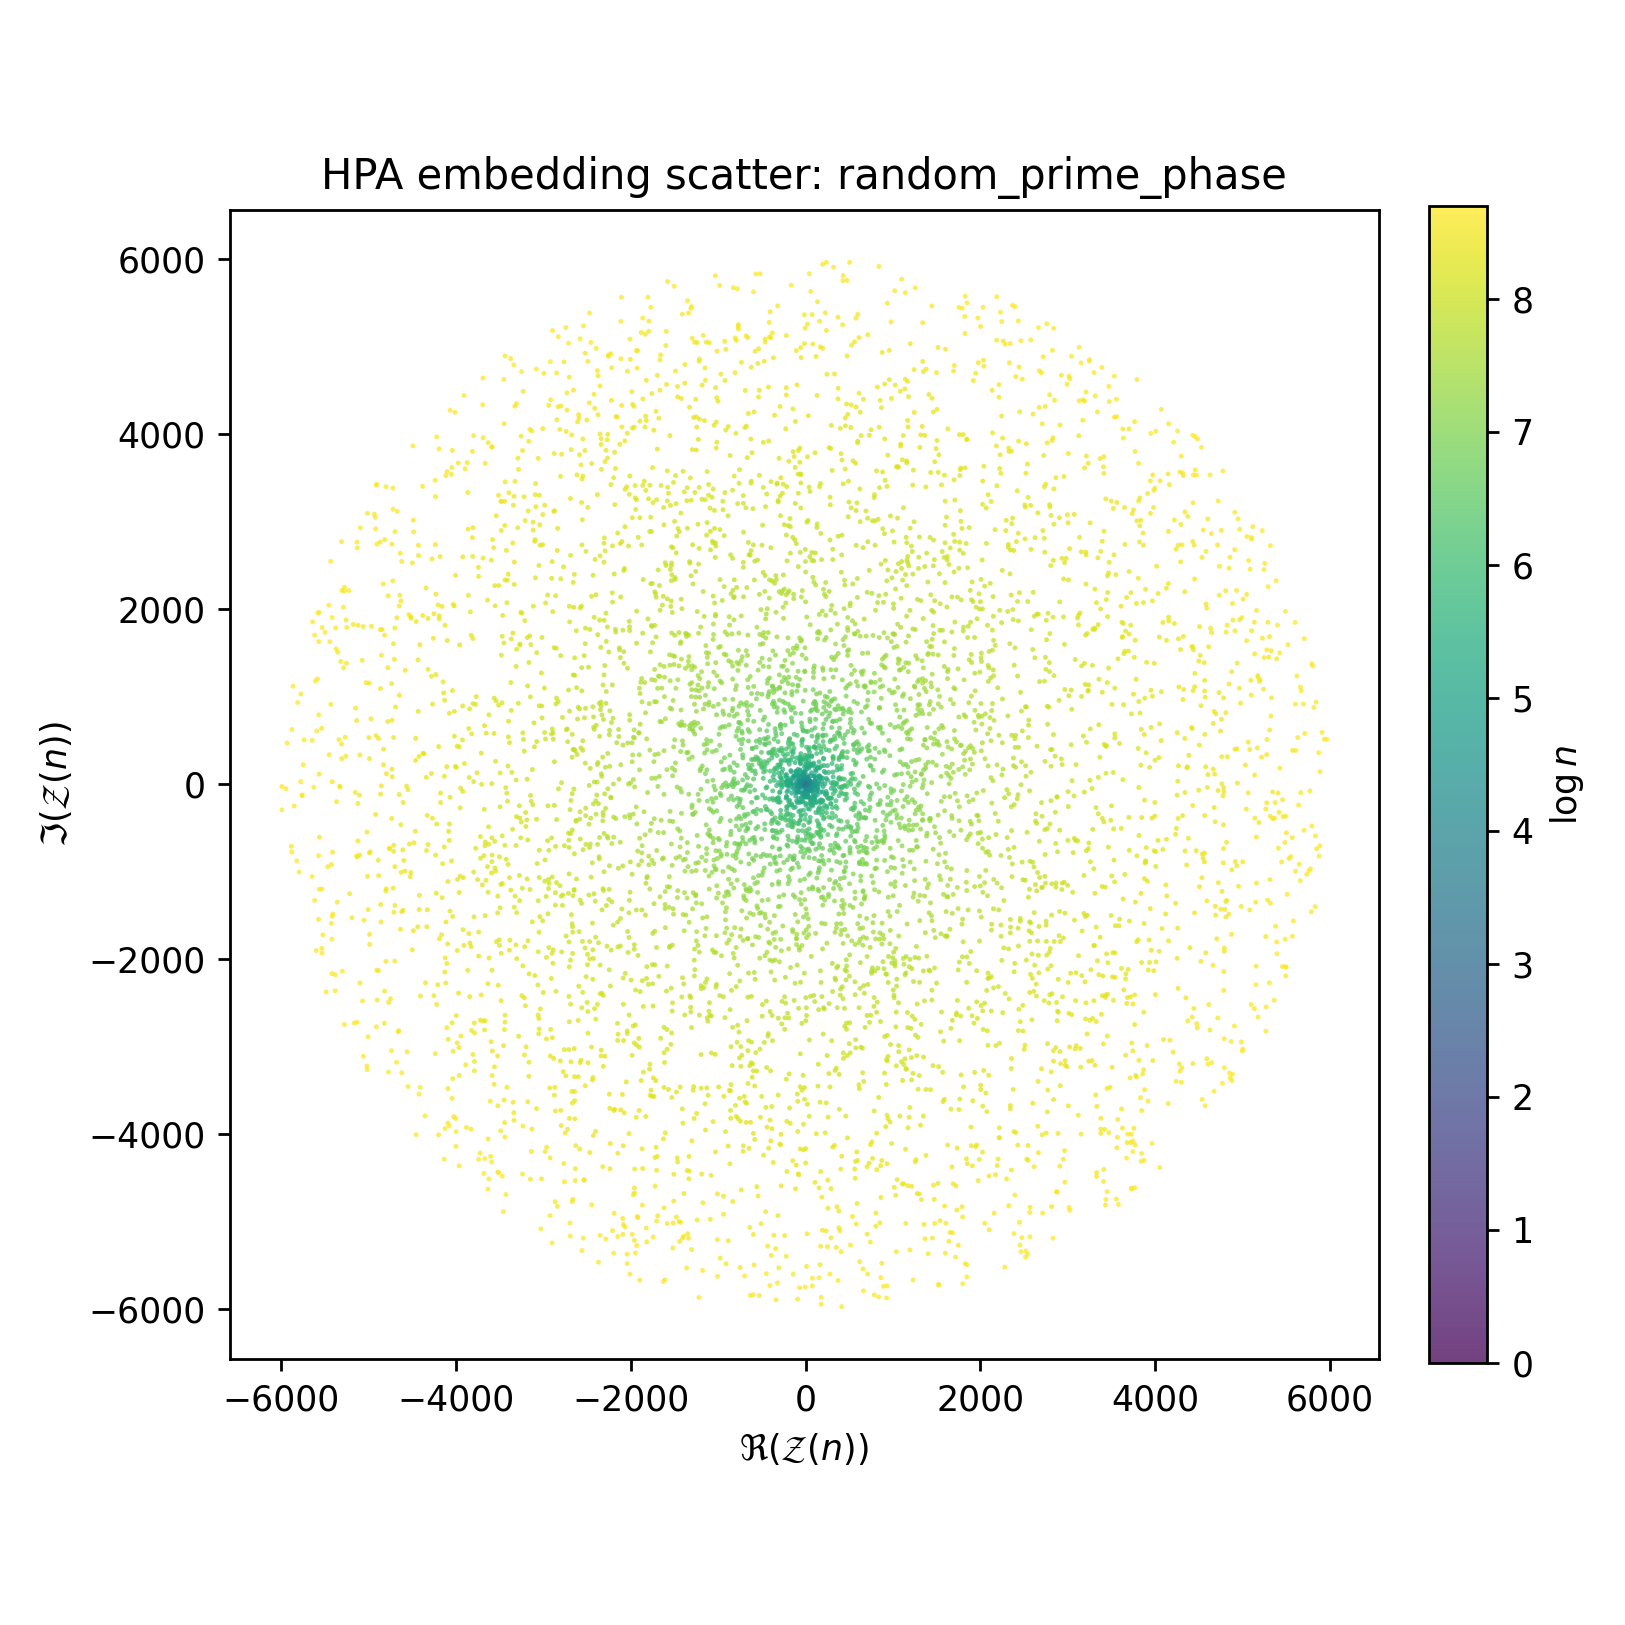
\includegraphics[width=0.32\textwidth]{images/hpa_Z_scatter_random_prime_phase.png}
    \caption{Scatter plots of $\mathcal{Z}(n)$ for $1\le n\le 6000$ under three phase models. Color encodes $\log n$.}
    \label{fig:hpa_scatter}
\end{figure}

\begin{figure}[t]
    \centering
    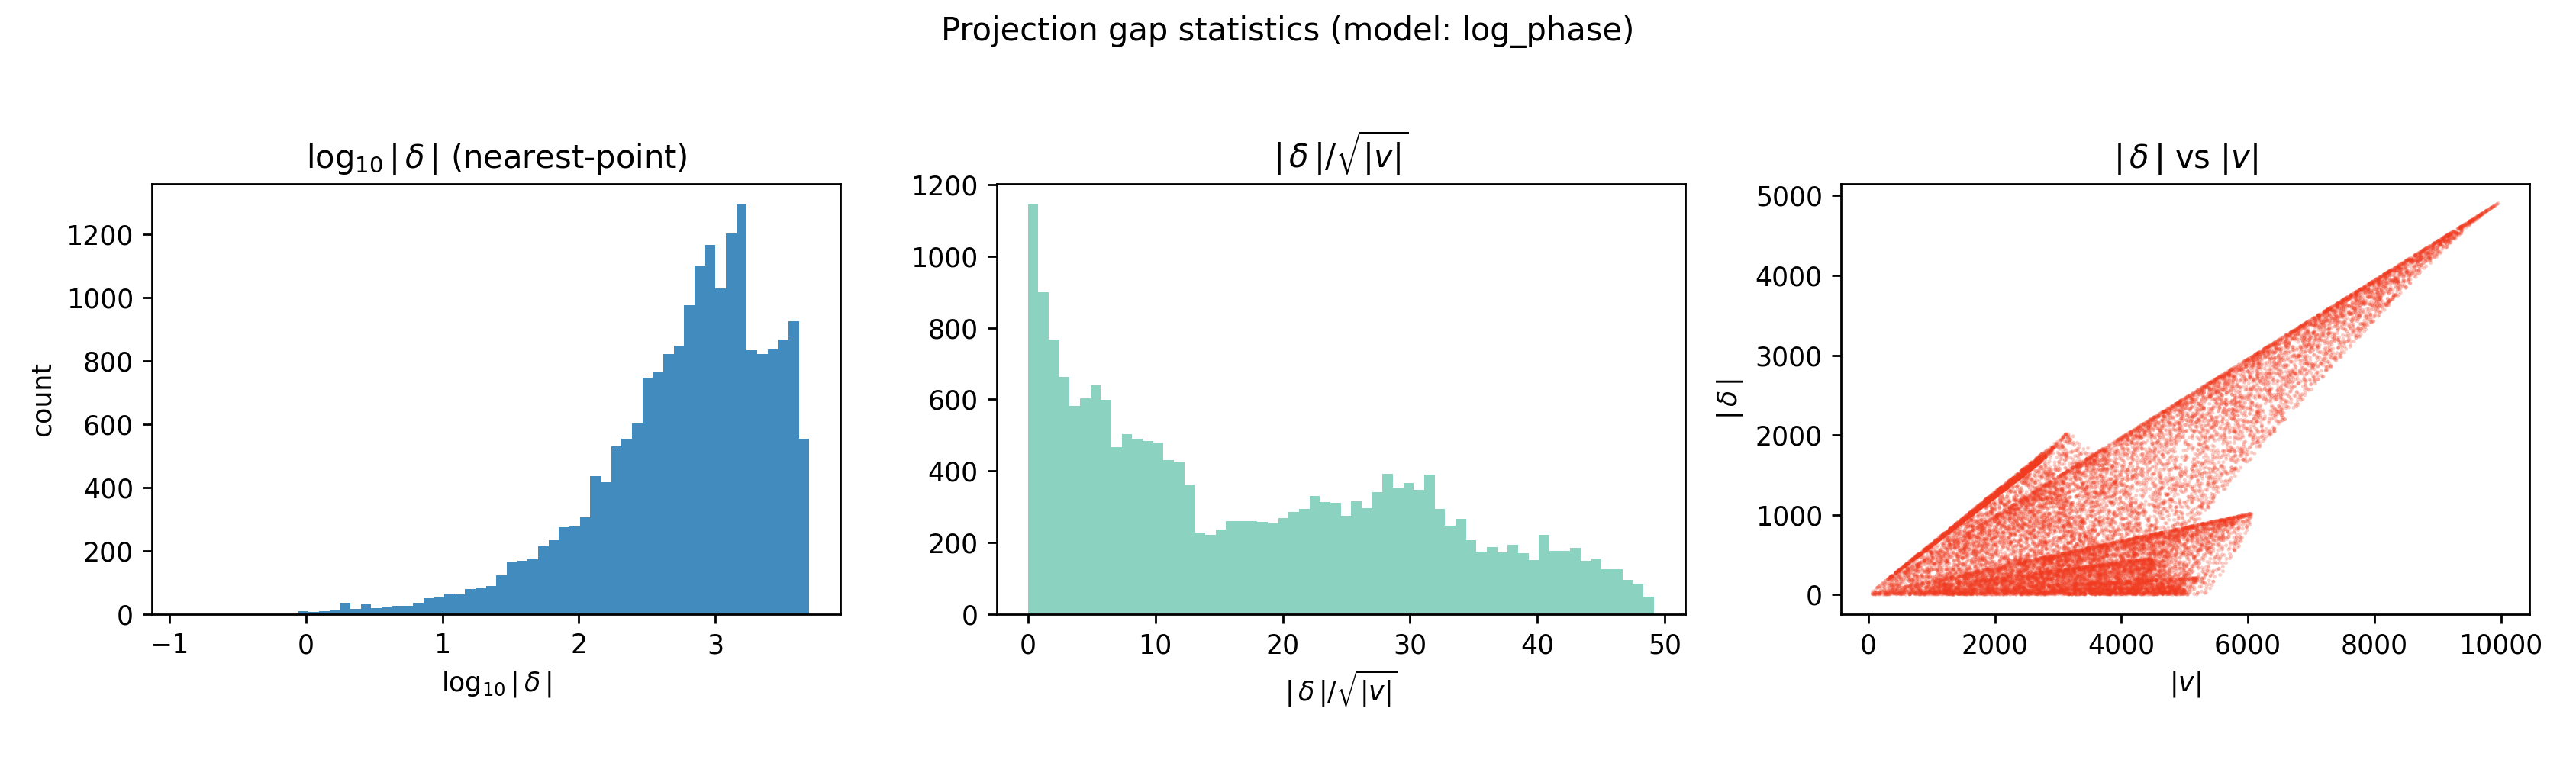
\includegraphics[width=0.32\textwidth]{images/hpa_gap_stats_log_phase.png}\hfill
    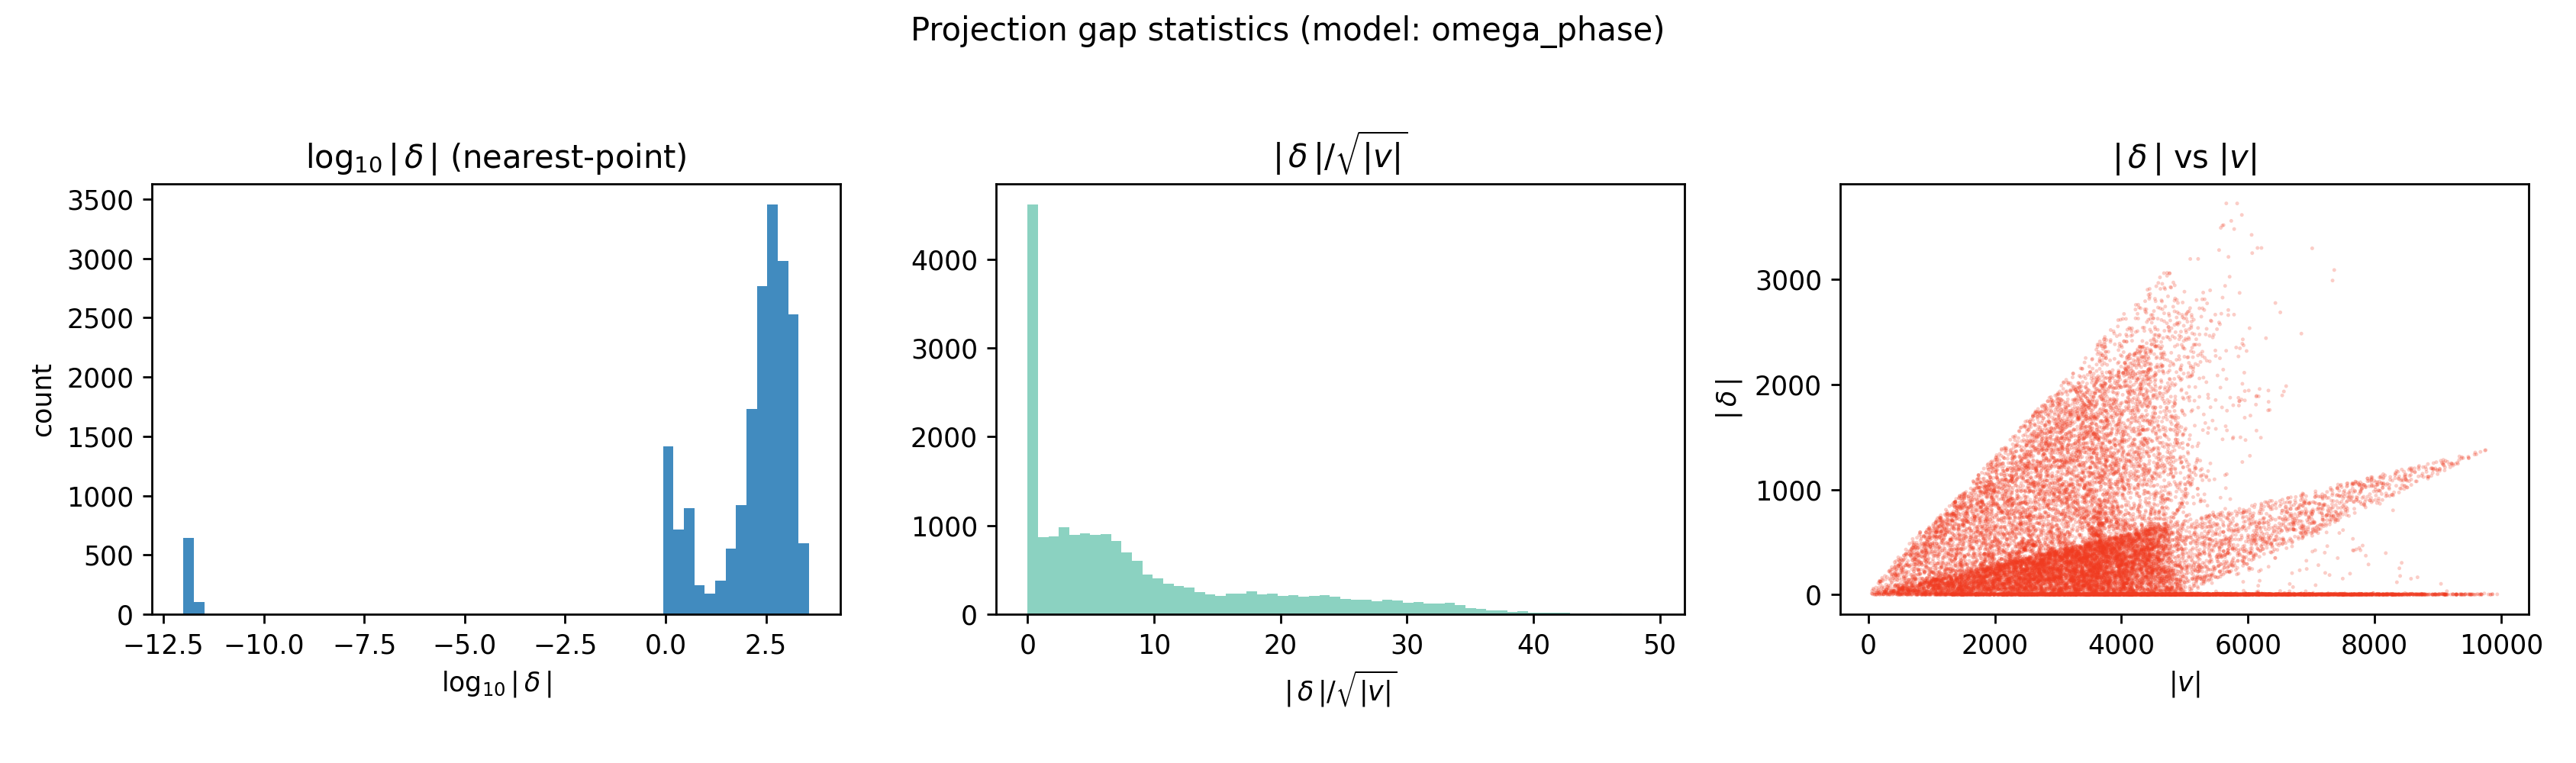
\includegraphics[width=0.32\textwidth]{images/hpa_gap_stats_omega_phase.png}\hfill
    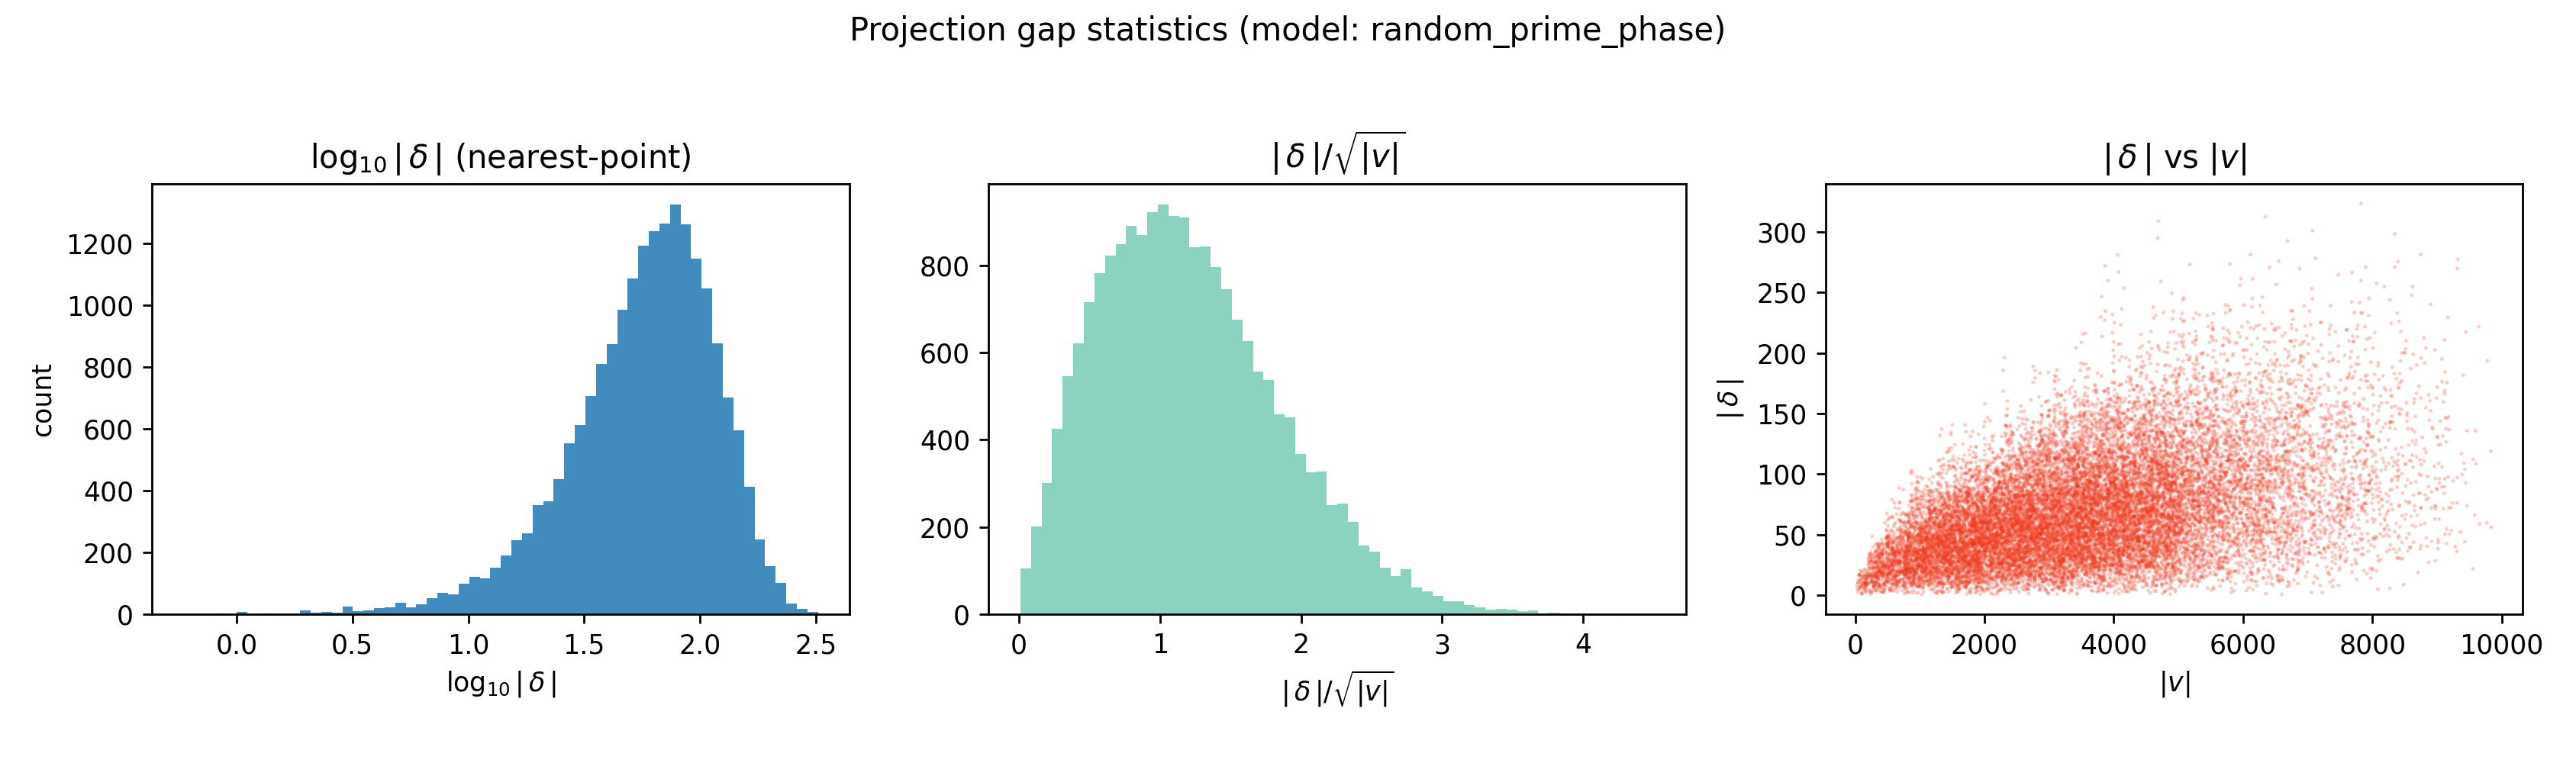
\includegraphics[width=0.32\textwidth]{images/hpa_gap_stats_random_prime_phase.png}
    \caption{Empirical projection-gap statistics for $v=\mathcal{Z}(a)+\mathcal{Z}(b)$ with $(a,b)$ uniform on $\{1,\dots,5000\}^2$ (20000 samples). Plots show $\log_{10}|\delta|$, the normalized gap $|\delta|/\sqrt{|v|}$, and a scatter of $|\delta|$ vs $|v|$.}
    \label{fig:hpa_gap_stats}
\end{figure}

\begin{figure}[t]
    \centering
    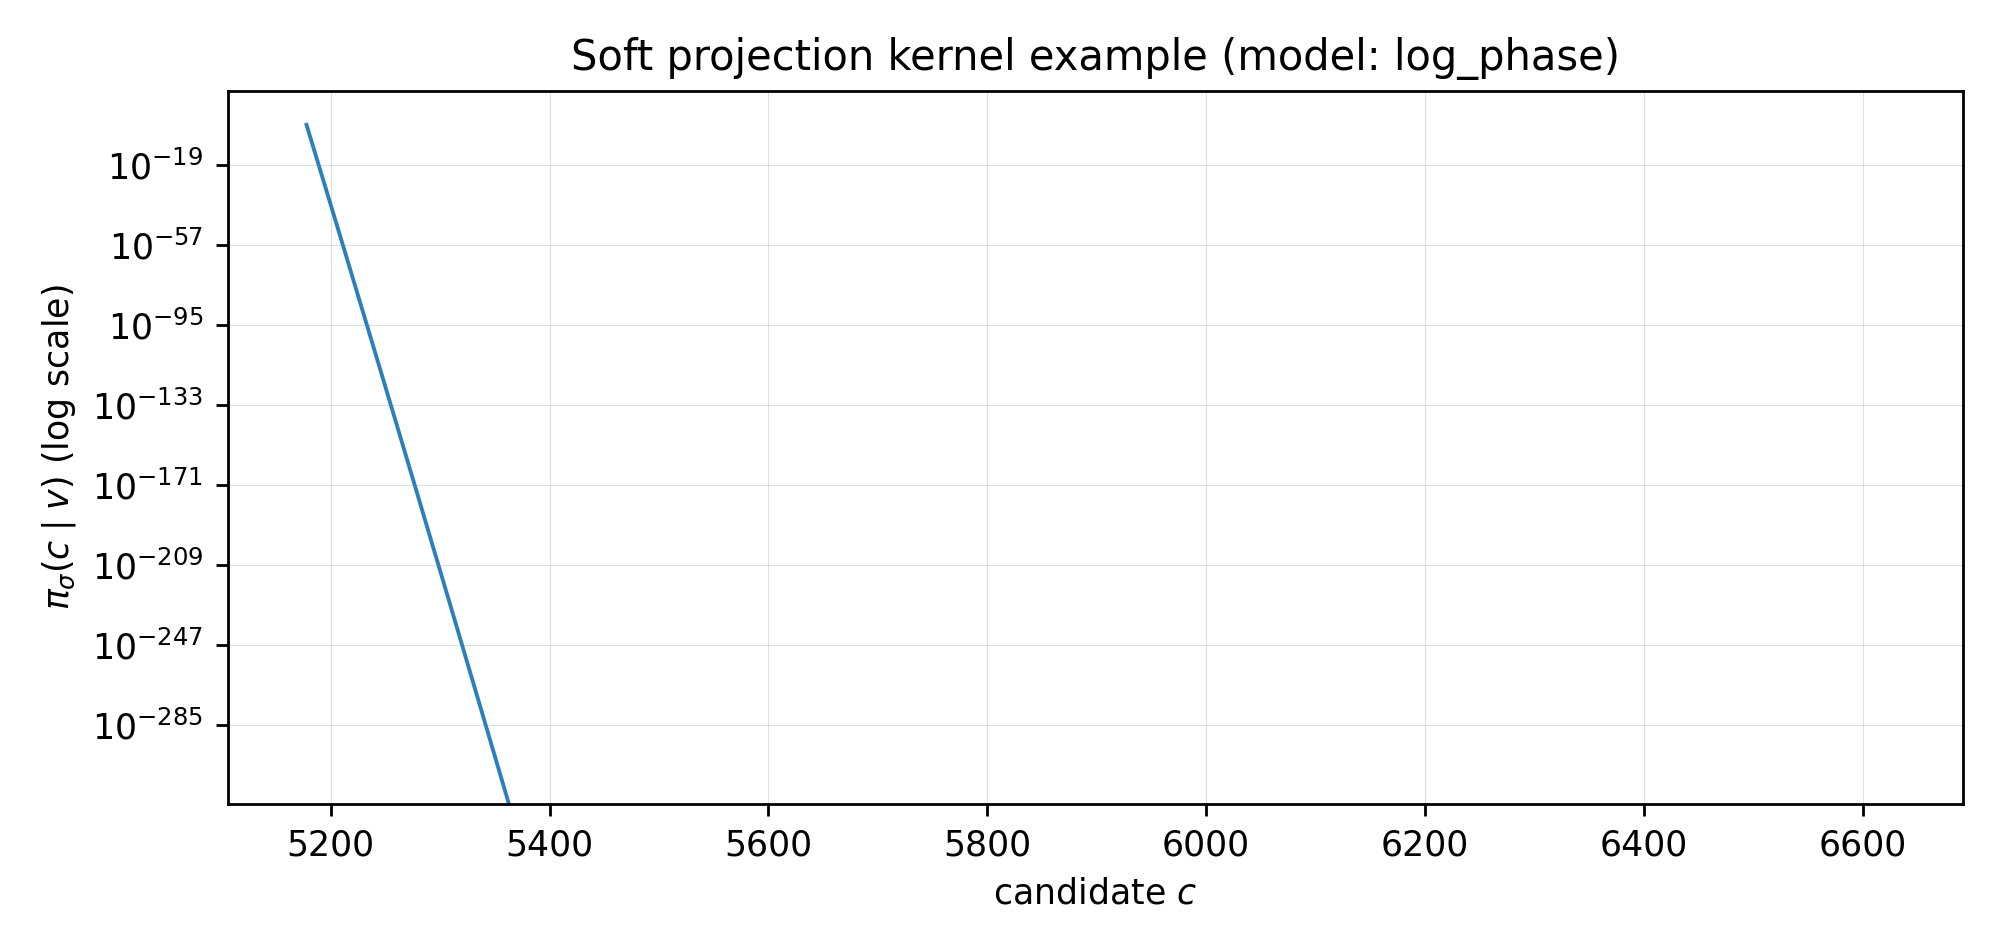
\includegraphics[width=0.32\textwidth]{images/hpa_kernel_example_log_phase.png}\hfill
    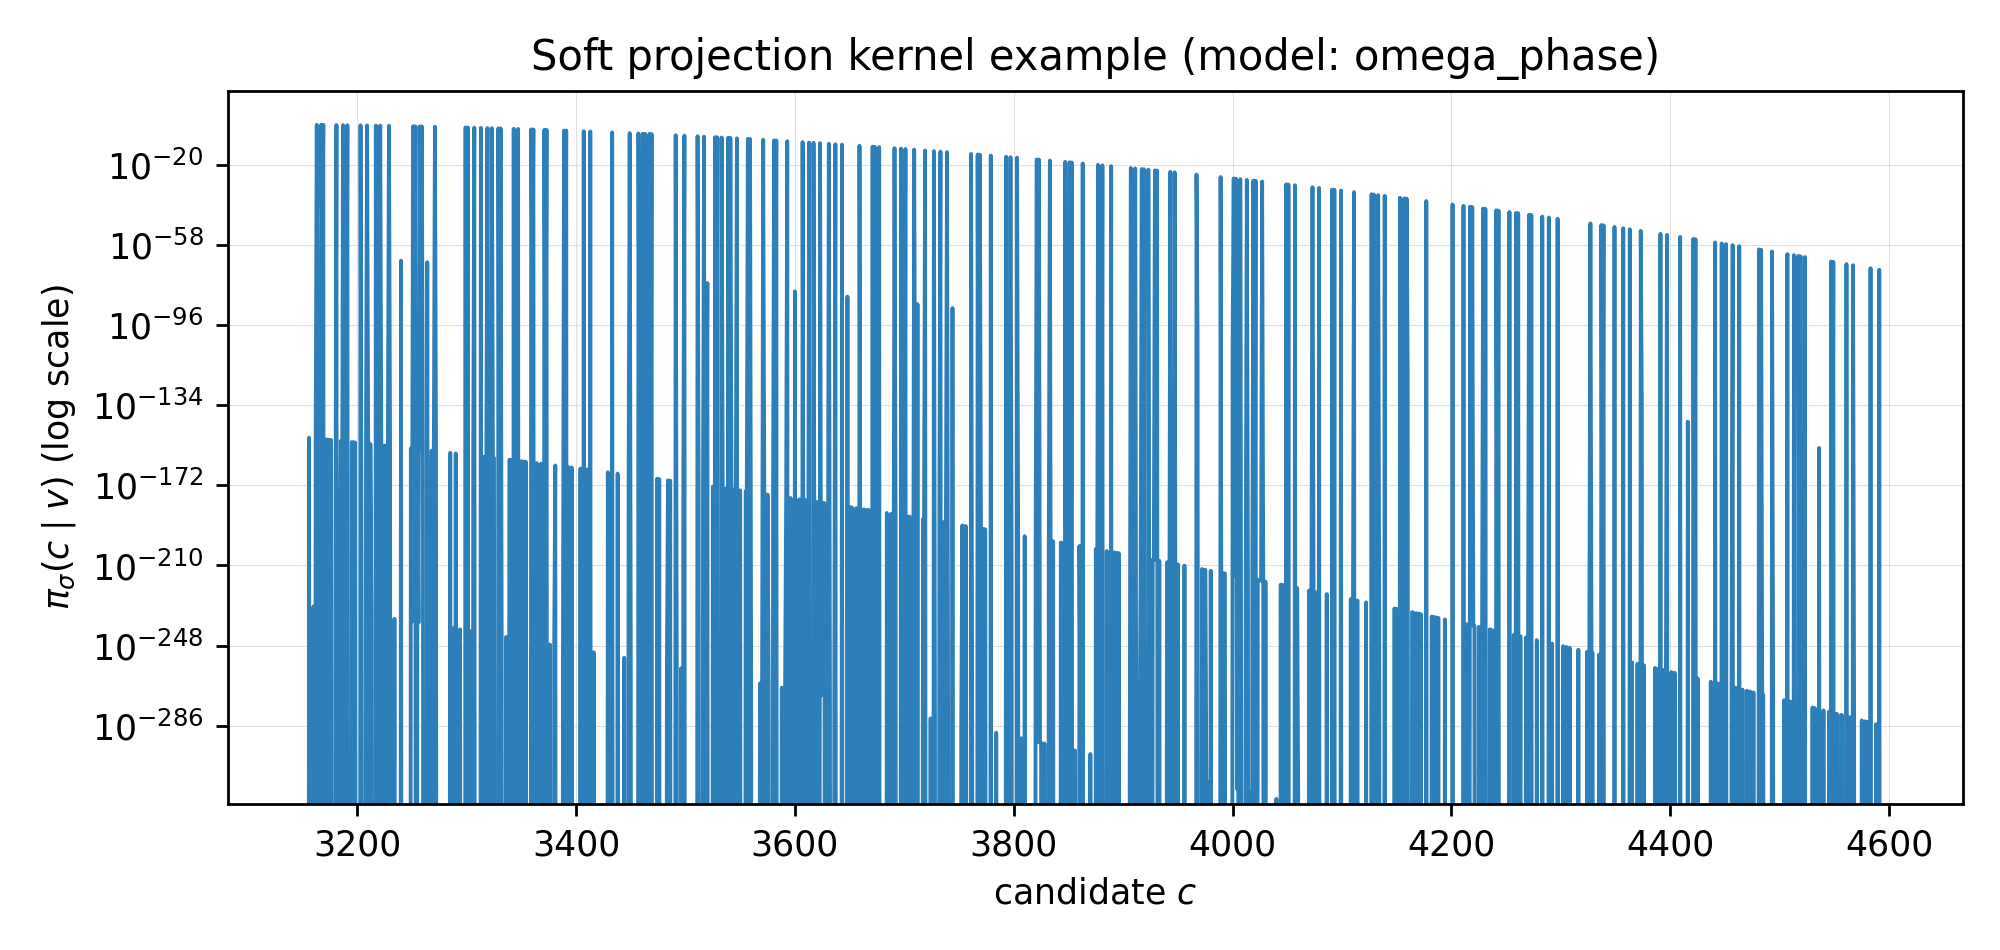
\includegraphics[width=0.32\textwidth]{images/hpa_kernel_example_omega_phase.png}\hfill
    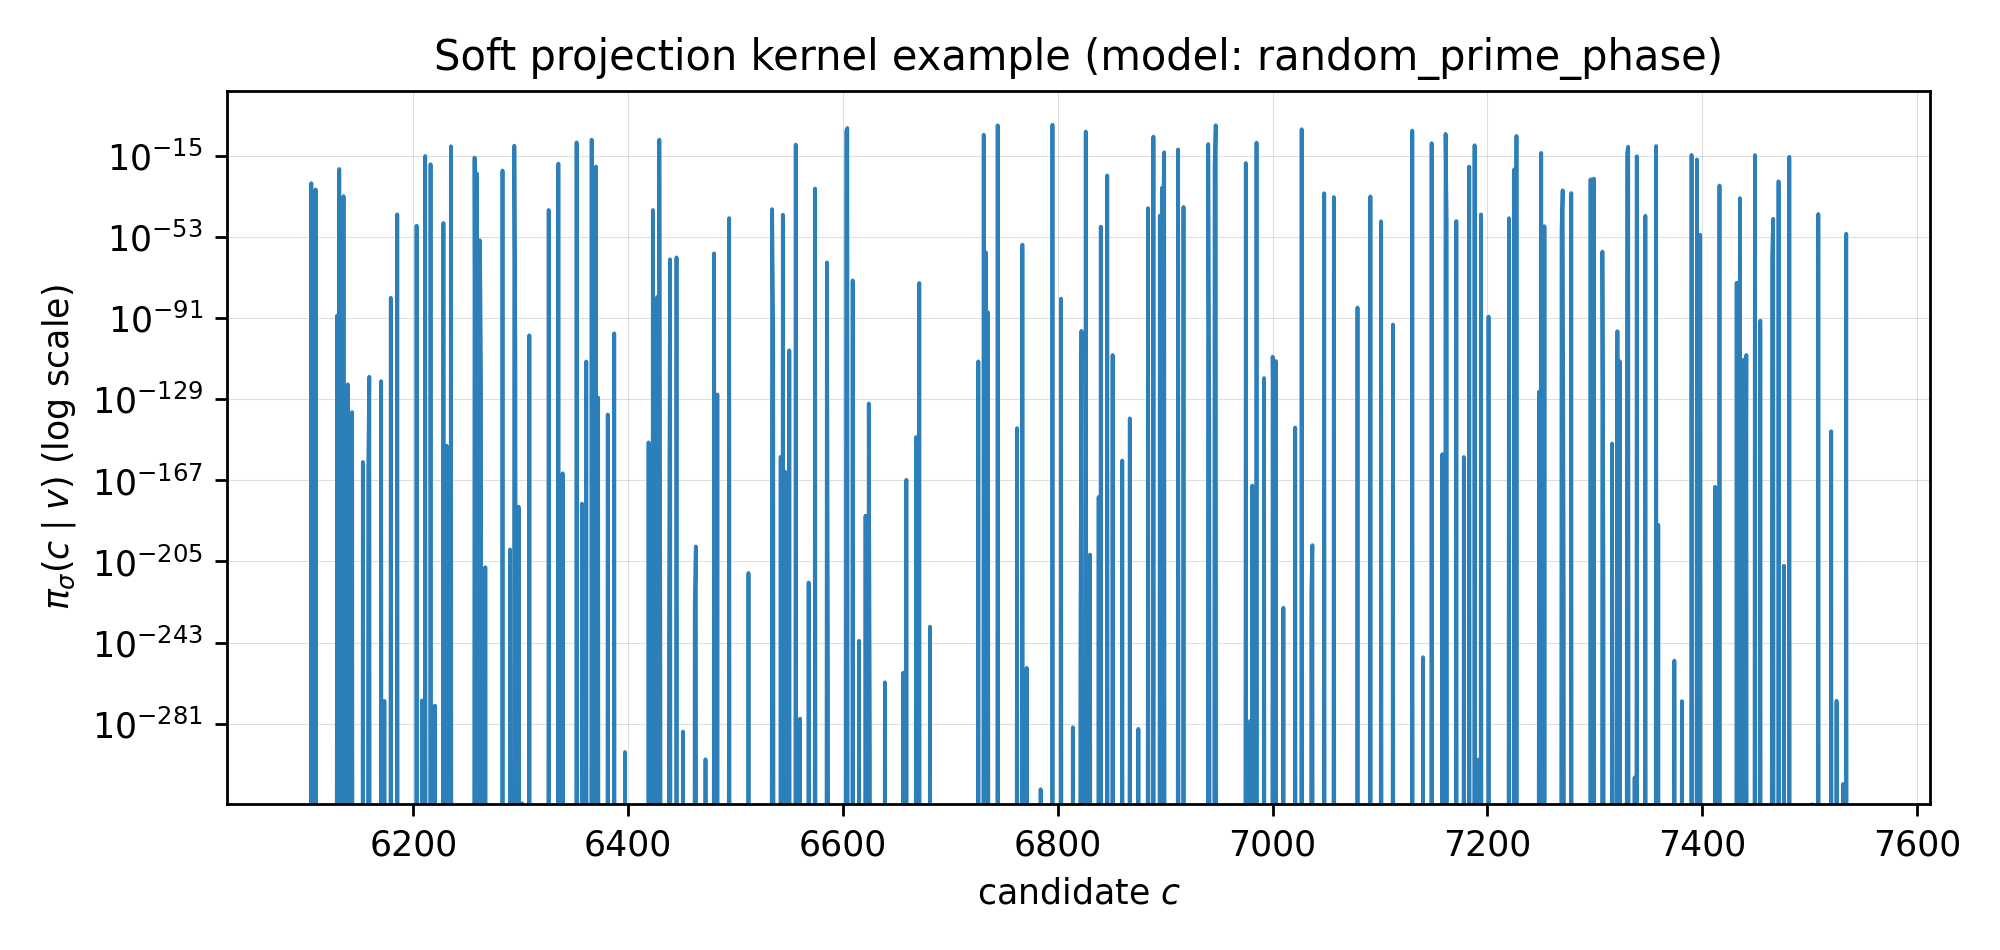
\includegraphics[width=0.32\textwidth]{images/hpa_kernel_example_random_prime_phase.png}
    \caption{Examples of the soft projection kernel $\pi_\sigma(\cdot\mid v)$ (Definition~\ref{def:projection_kernel}) for $v=\mathcal{Z}(3000)+\mathcal{Z}(4000)$ with $\sigma=120$, plotted on a logarithmic vertical scale.}
    \label{fig:hpa_kernel_example}
\end{figure}

\paragraph{Readout stability under window perturbations.}
For the golden slope $\alpha=\varphi^{-1}$ and window $W=[1-\alpha,1)$, we compare the readout with its shifted-window variant $W_\eta=[1-\alpha+\eta,1+\eta)$ (mod $1$), over $N=4000$ scan steps and $200$ random intercepts $x_0$.
Figure~\ref{fig:hpa_readout_stability} reports the mean flip rate and the induced changes in the prefix count $S_N$ and its Zeckendorf coding.

\begin{figure}[t]
    \centering
    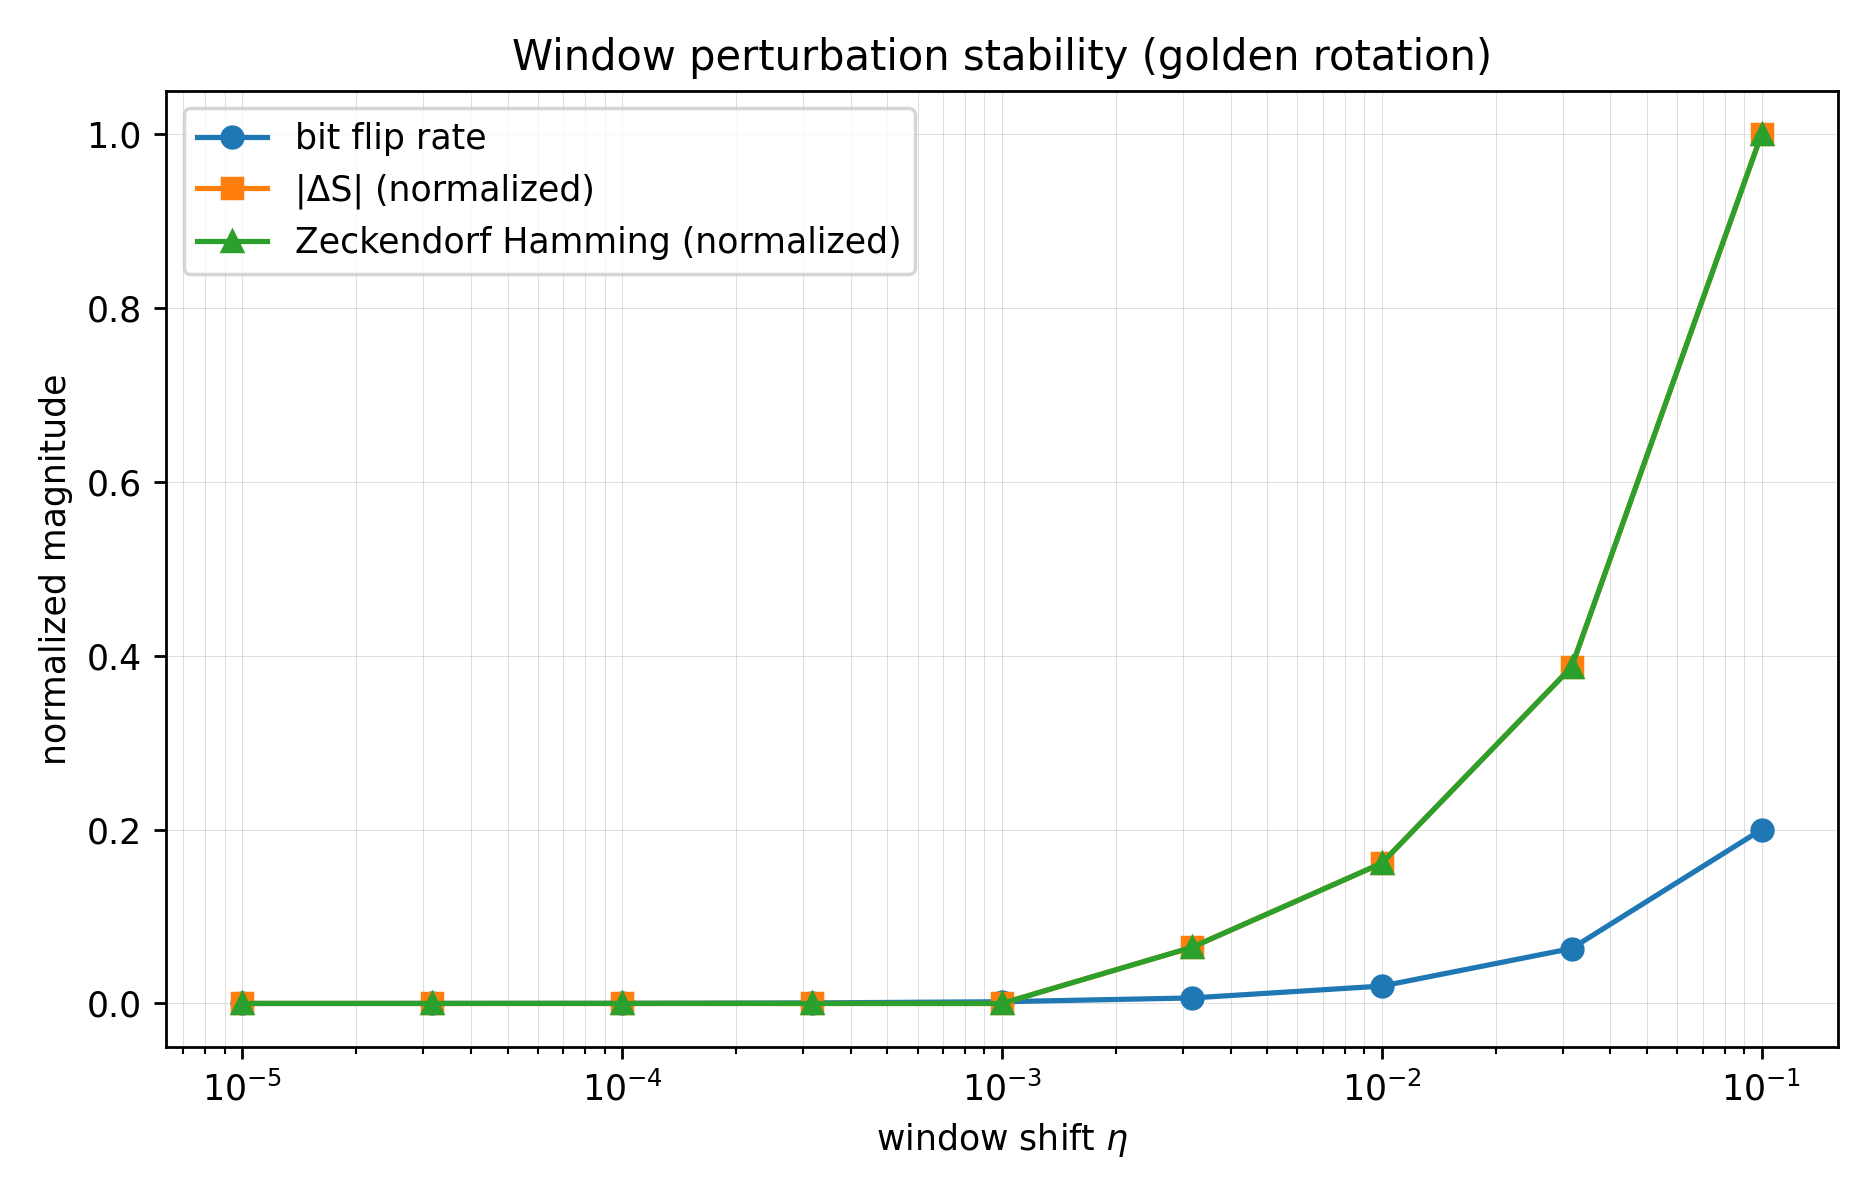
\includegraphics[width=0.7\textwidth]{images/hpa_readout_stability_golden.png}
    \caption{Empirical stability of golden-rotation readout under window shifts $\eta\in[10^{-5},10^{-1}]$: mean bit flip rate, and normalized changes in $|S_N-S_N'|$ and Zeckendorf code Hamming distance.}
    \label{fig:hpa_readout_stability}
\end{figure}

\begin{figure}[t]
    \centering
    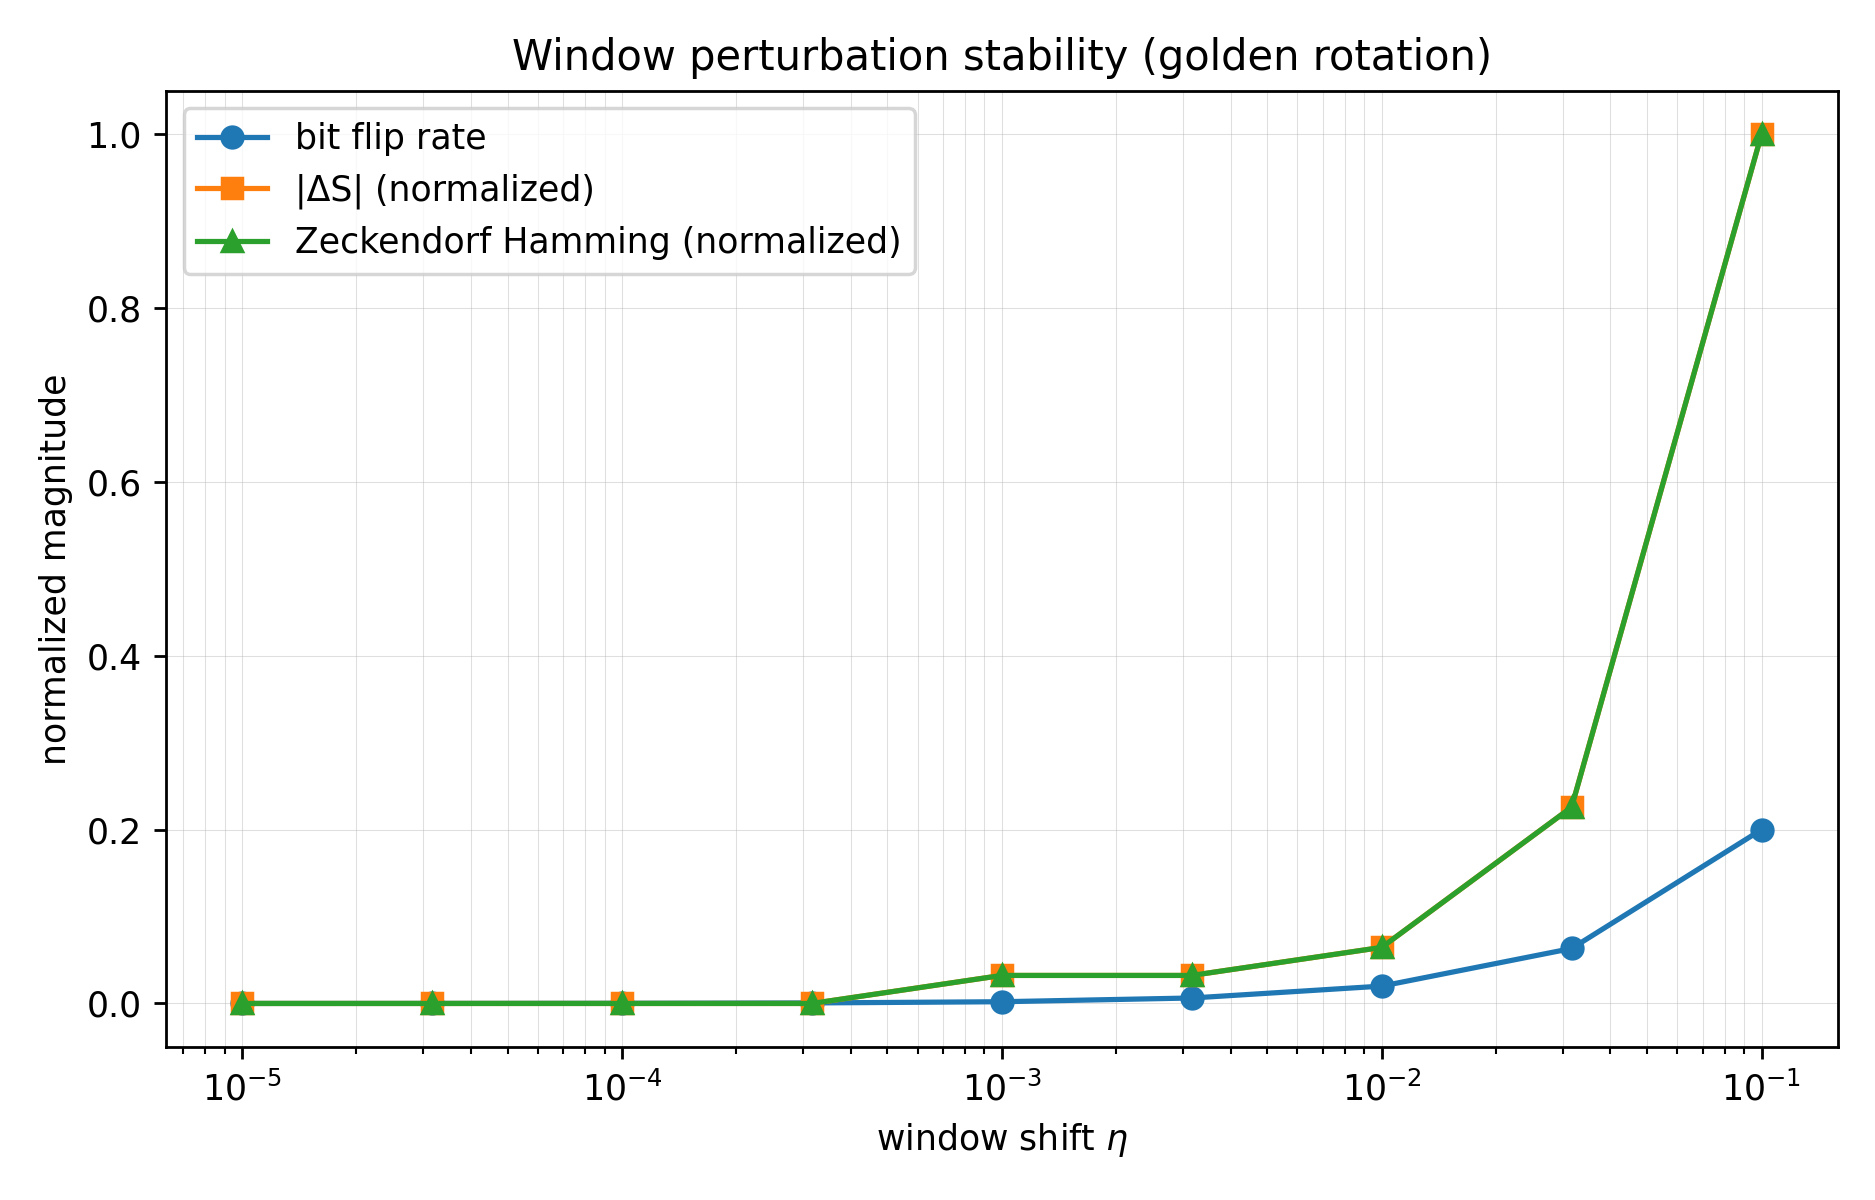
\includegraphics[width=0.7\textwidth]{images/hpa_readout_stability_silver.png}
    \caption{An Ostrowski (non-golden) comparison: $\alpha=\sqrt{2}-1=[0;2,2,2,\dots]$ with the same window shift experiment as in Figure~\ref{fig:hpa_readout_stability}, and code distance measured in the corresponding Ostrowski digits.}
    \label{fig:hpa_readout_stability_silver}
\end{figure}
